% Hier folgt der Inhalt des Abschnitts "Anhang".

\subsection{Pinbelegung}

\begin{figure}[ht]
  \centering
  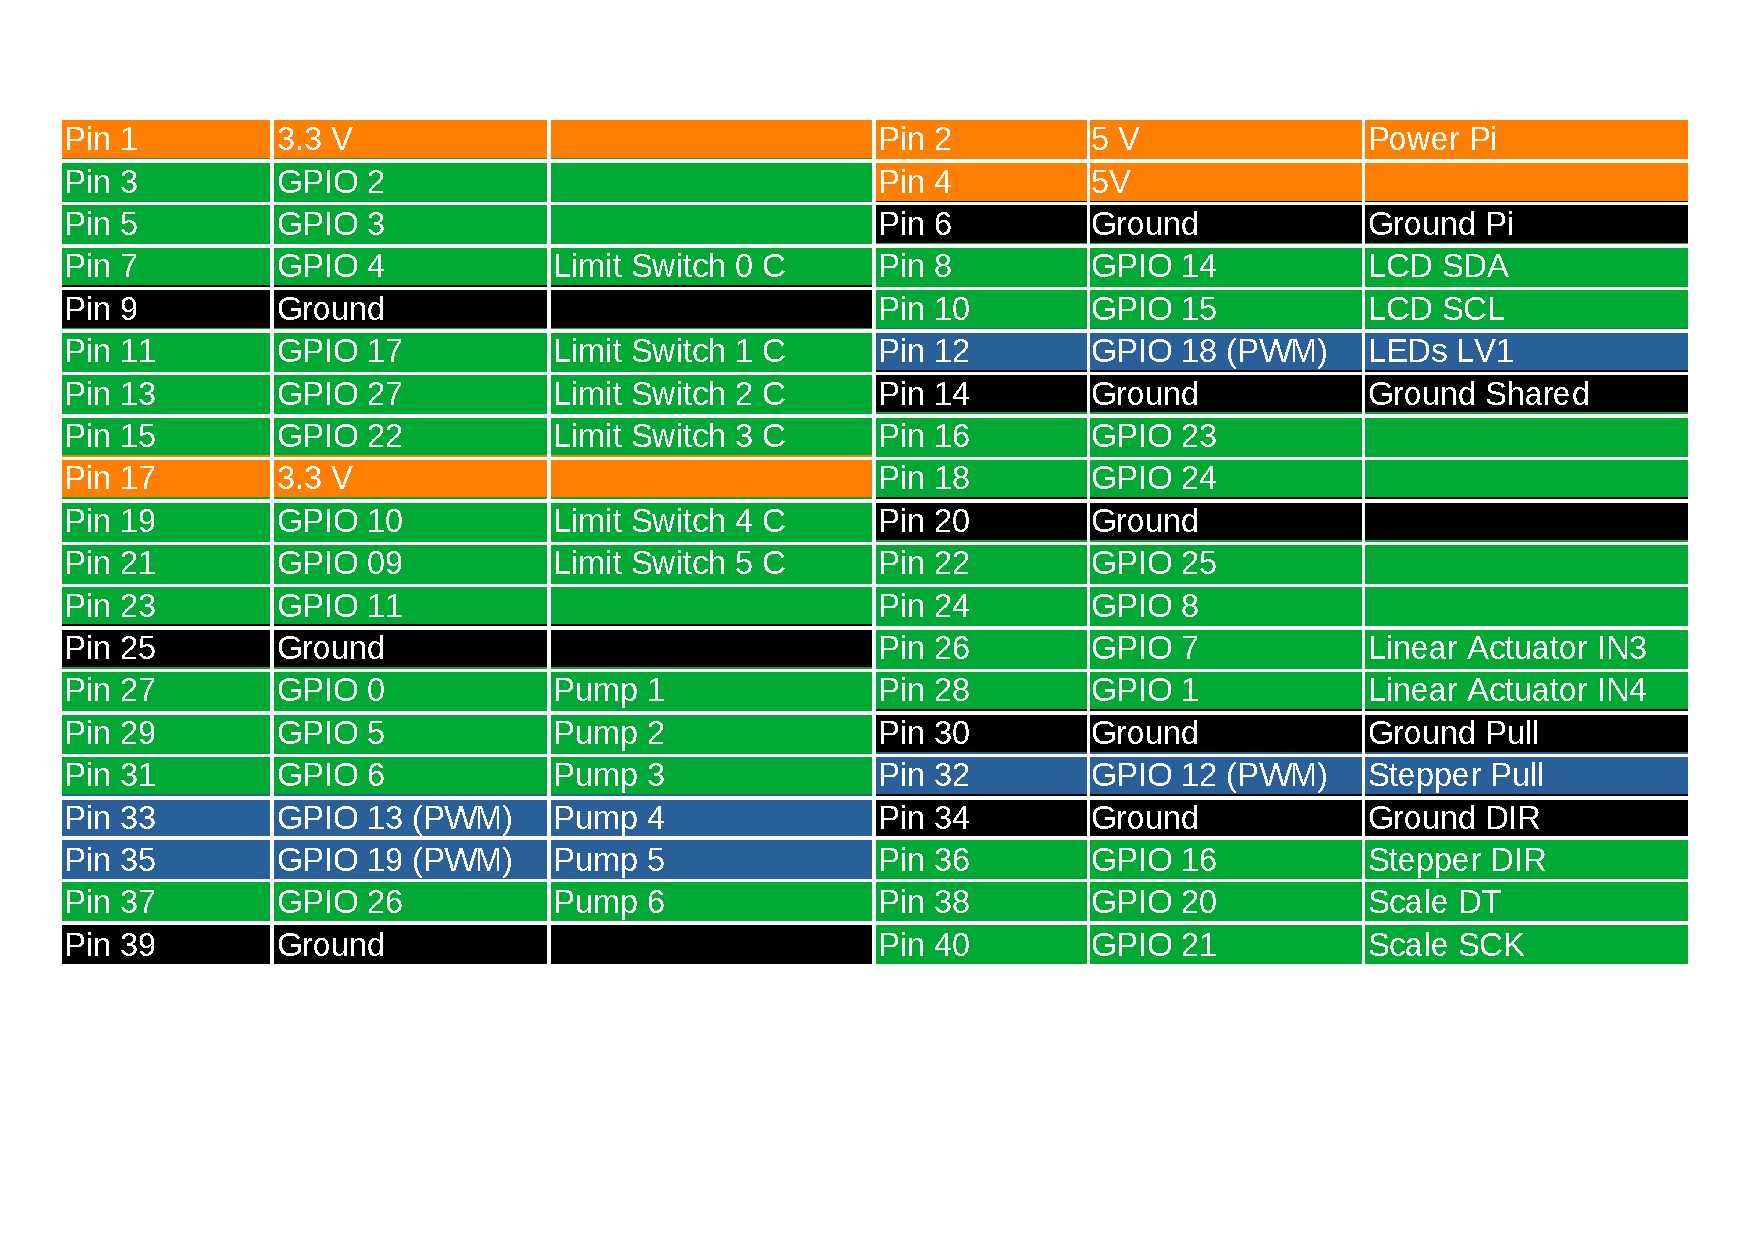
\includegraphics[width=\textwidth]{graphics/images/pinning_final.pdf}
  \caption{Pinbelegung des Rapsberry Pi Zero 2 W}
  \label{fig:pinning}
\end{figure}

\newpage

\subsection{Schaltplan}

\begin{figure}[ht]
  \centering
  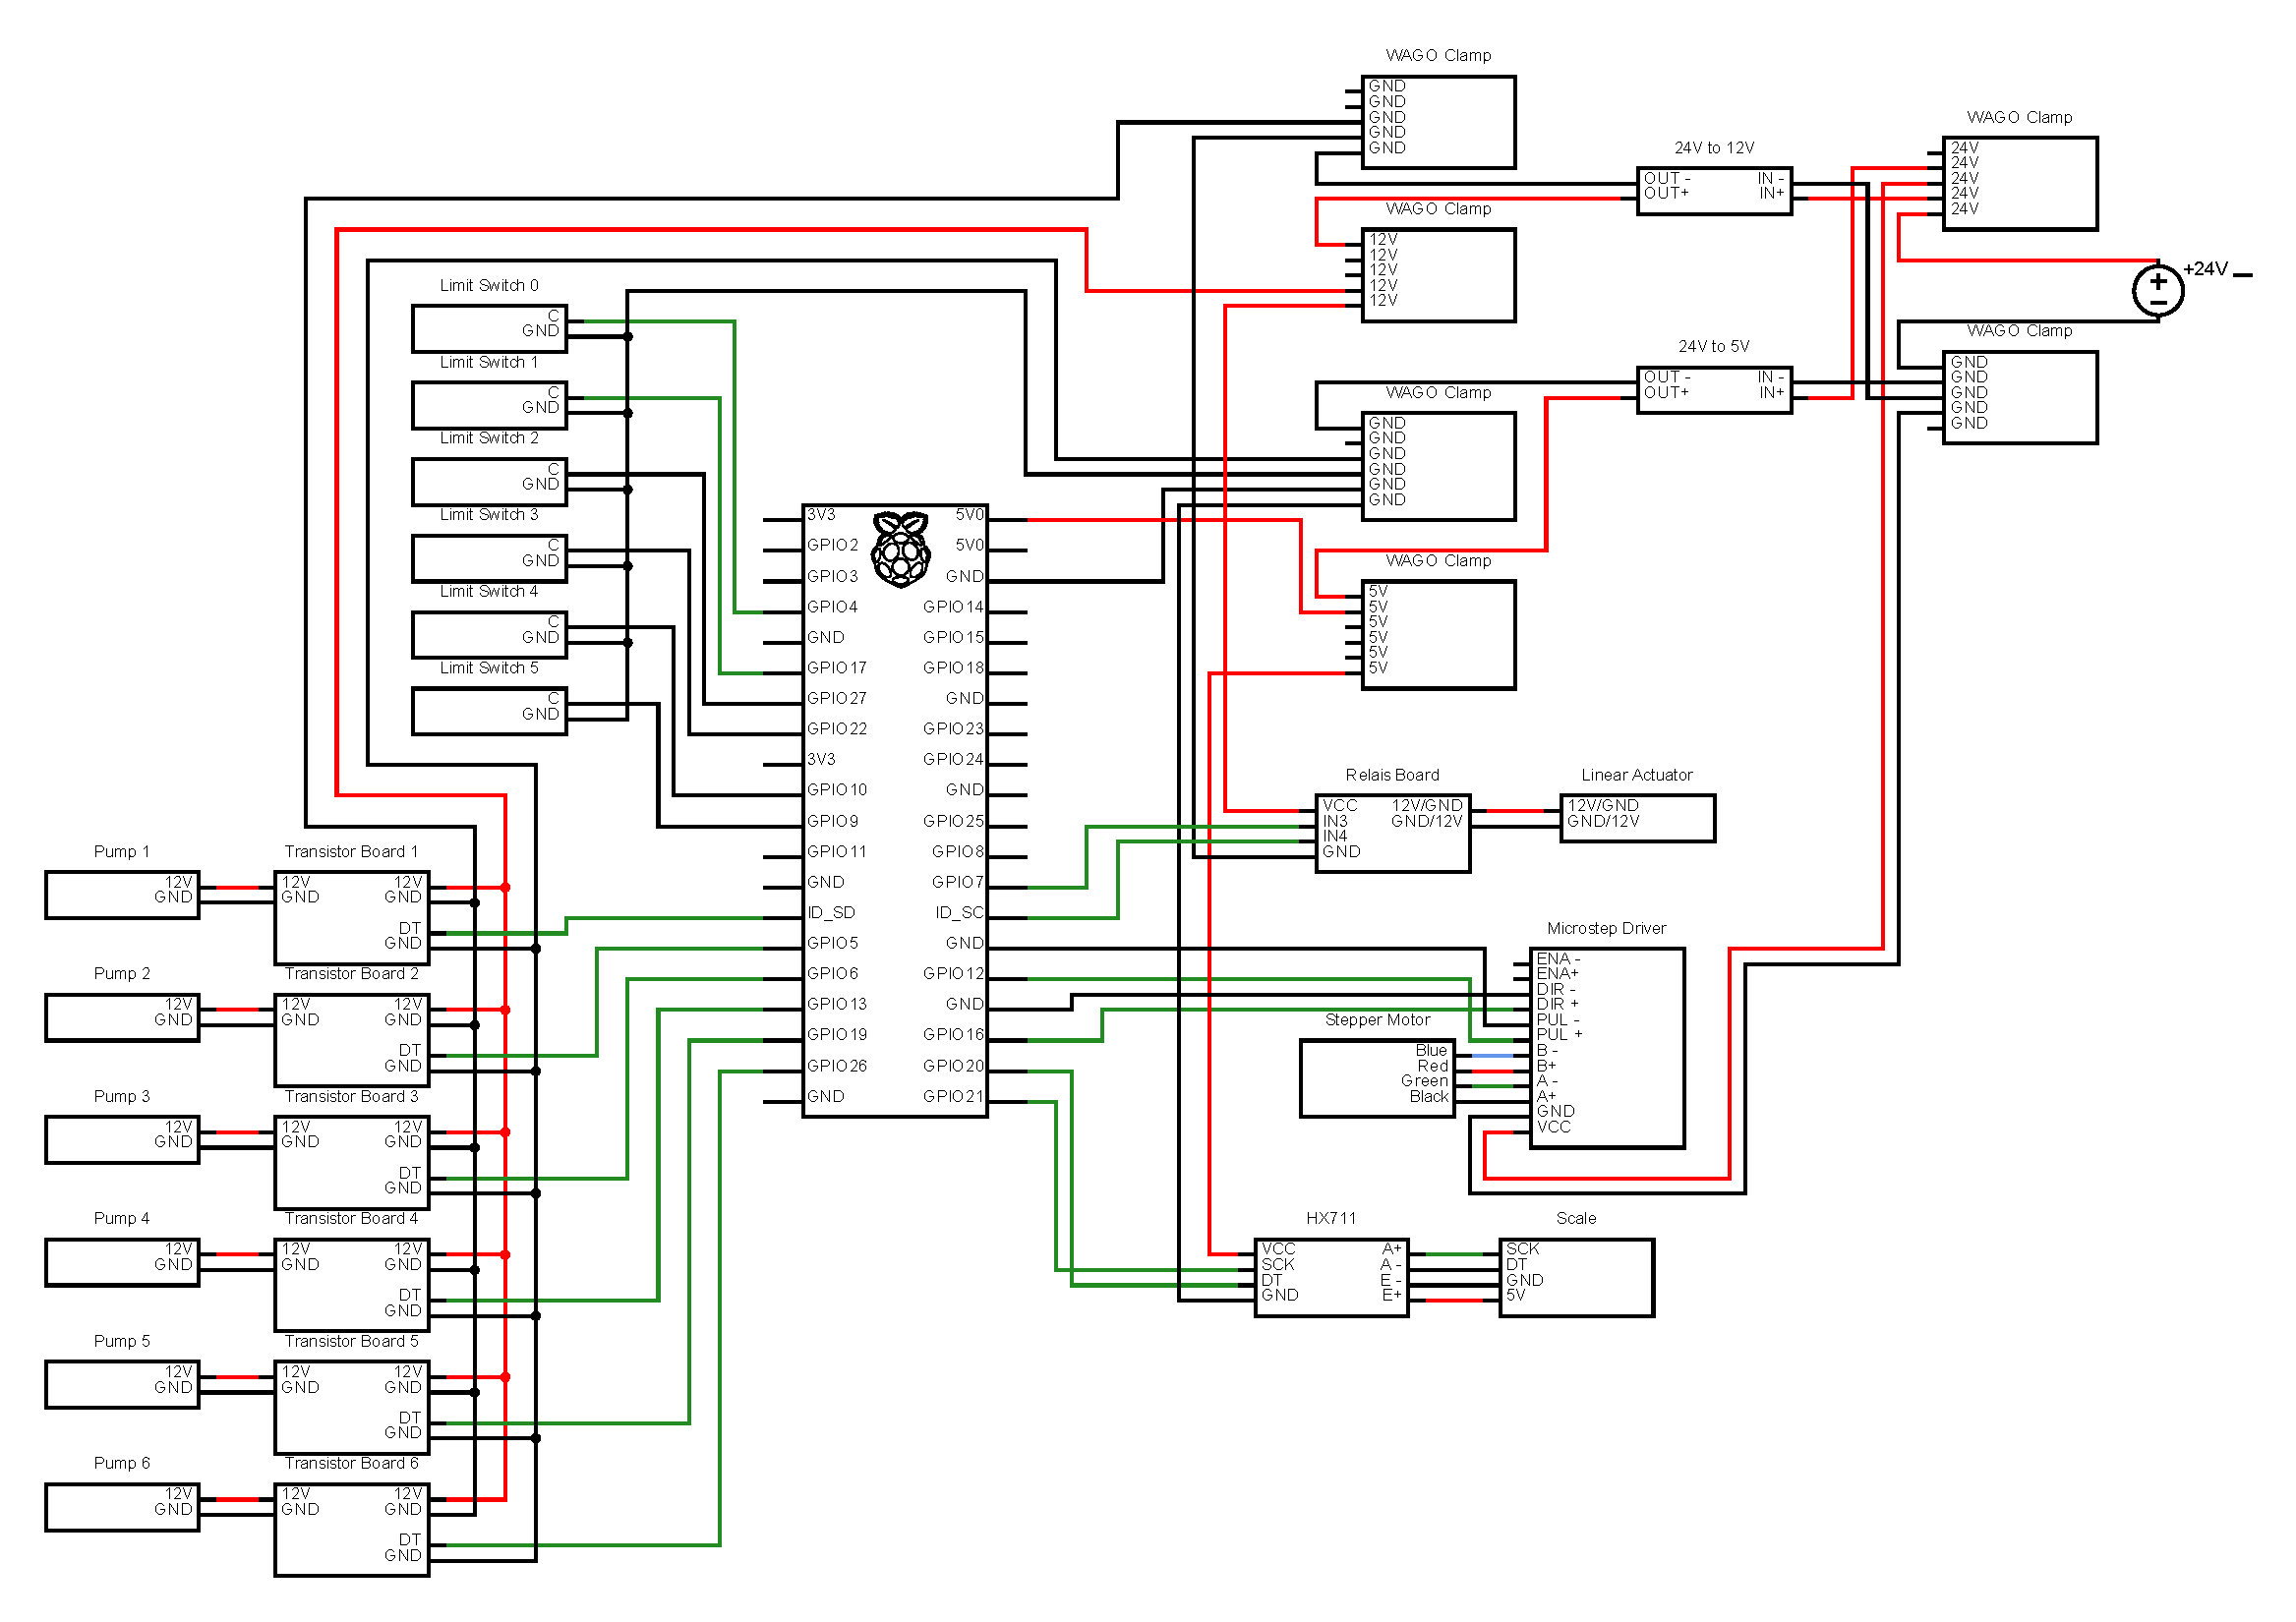
\includegraphics[height=0.84\textwidth, angle=270]{graphics/images/schaltplan.pdf}
  \caption{Schaltplan der Hardwarekomponenten}
  \label{fig:schaltplan}
\end{figure}

\newpage
\subsection{Datenbankdiagramm}

\begin{figure}[H]
  \centering
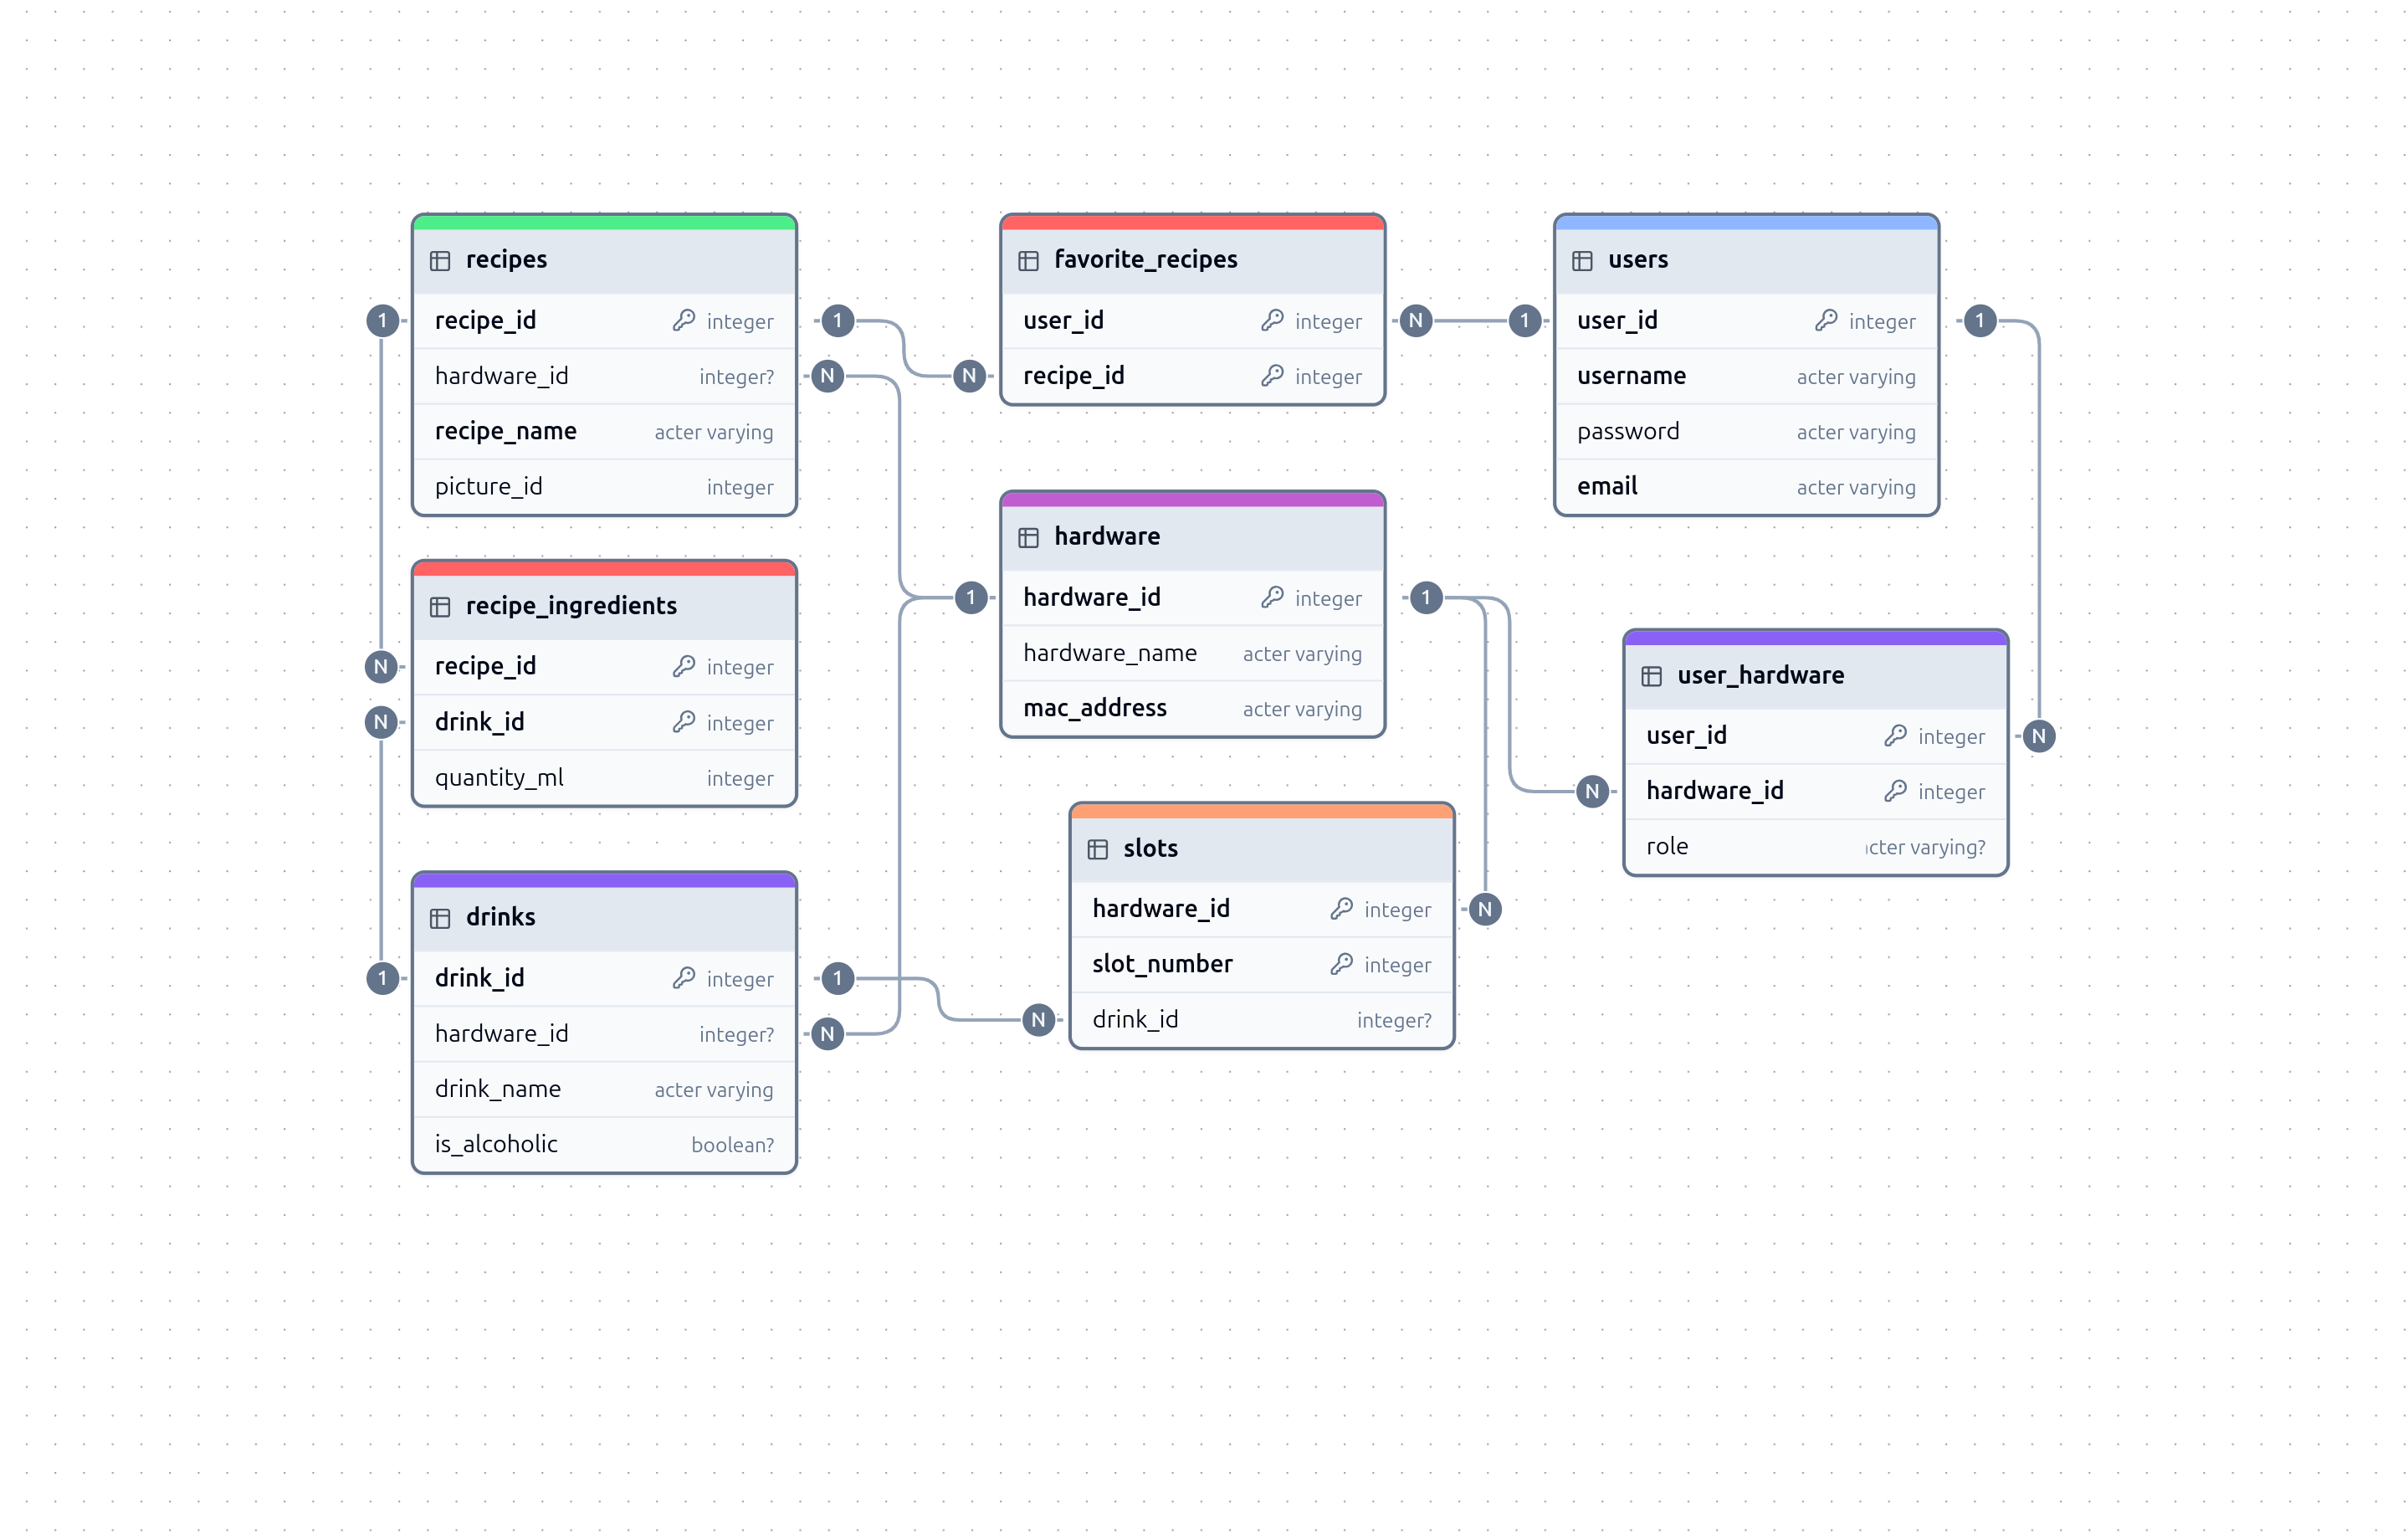
\includegraphics[height=0.96\textwidth, angle=270]{graphics/schemes/postgres_db_scheme.png}
  \caption{Datenbankdiagramm}
  \label{fig:database_diagram}
\end{figure}

\subsection{Pinbelegung Tabelle}
\newpage
\begin{figure}[H]
  \footnotesize
  \begin{tabularx}{\textwidth}{|l|X|X|l|X|X|}
    \hline
    \textbf{PINS} & \textbf{INFO} & \textbf{USAGE} & \textbf{PINS} & \textbf{INFO} & \textbf{USAGE} \\
    \hline
    Pin 1 & 3.3 V & & Pin 2 & 5 V & \\
    \hline
    Pin 3 & GPIO 2 & & Pin 3 & 5 V & \\
    \hline
    Pin 5 & GPIO 3 & & Pin 6 & Ground & Ground for Pi \\
    \hline
    Pin 7 & GPIO 4 & Limit Switch 1 C & Pin 8 & GPIO 14 & LCD SDA \\
    \hline
    Pin 9 & Ground & & Pin 10 & GPIO 15 & LCD SCL \\
    \hline
    Pin 11 & GPIO 17 & Limit Switch 2 C & Pin 12 & GPIO 18 (PWM) & LED LV1 \\
    \hline
    Pin 13 & GPIO 27 & Limit Switch 3 C & Pin 14 & Ground & Shared Ground \\
    \hline
    Pin 15 & GPIO 22 & Limit Switch 4 C & Pin 16 & GPIO 23 & \\
    \hline
    Pin 17 & 3.3 V & & Pin 18 & GPIO 24 & \\
    \hline
    Pin 19 & GPIO 10 & Limit Switch 5 C & Pin 20 & Ground & \\
    \hline
    Pin 21 & GPIO 9 & Limit Switch 6 C & Pin 22 & GPIO 25 & Actuator IN1 \\
    \hline
    Pin 23 & GPIO 11 & Limit Switch 7 C & Pin 24 & GPIO 8 & Actuator IN2 \\
    \hline
    Pin 25 & Ground & & Pin 26 & GPIO 7 & Actuator IN3 \\
    \hline
    Pin 27 & GPIO 0 & Pump 1 & Pin 28 & GPIO 1 & Actuator IN4 \\
    \hline
    Pin 29 & GPIO 5 & Pump 2 & Pin 30 & Ground & \\
    \hline
    Pin 31 & GPIO 6 & Pump 3 & Pin 32 & GPIO 12 (PWM) & Stepper DA \\
    \hline
    Pin 33 & GPIO 13 (PWM) & Pump 4 & Pin 34 & Ground & Ground Stepper \\
    \hline
    Pin 35 & GPIO 19 (PWM) & Pump 5 & Pin 36 & GPIO 16 & Stepper Dir \\
    \hline
    Pin 37 & GPIO 26 & Pump 6 & Pin 38 & GPIO 20 & Scale DT \\
    \hline
    Pin 39 & Ground & & Pin 40 & GPIO 21 & Scale SCK \\
    \hline
  \end{tabularx}
  \normalsize
  \caption{Raspberry Pi 2 GPIO-Pinbelegung}
  \label{fig:raspberry_pi_pinout_tabularx}
\end{figure}
  
\newpage
\subsection{Weiterer Anhang}

\subsection{k6 Testskript}
\begin{lstlisting}[language=JavaScript]
  import http from 'k6/http';
  import { check, sleep } from 'k6';
  import { Counter } from 'k6/metrics';
  
  export let errorCounter = new Counter('errors');
  
  export const options = {
    stages: [
      { duration: '1m', target: 1 }, // 1 Nutzer
      { duration: '1m', target: 2 }, // 2 Nutzer
      { duration: '1m', target: 4 }, // 4 Nutzer
      { duration: '1m', target: 5 }, // 5 Nutzer
      { duration: '1m', target: 20 }, // 20 Nutzer
    ],
  };
  
  const BASE_URL = 'https://smartender-432708816033.europe-west3.run.app';
  const API_KEY = 'b0ec1aa3-98bd-434d-b6b6-f72b99383859';
  
  function randomString(length) {
    const chars = 'abcdefghijklmnopqrstuvwxyz1234567890';
    let result = '';
    for (let i = 0; i < length; i++) {
      result += chars.charAt(Math.floor(Math.random() * chars.length));
    }
    return result;
  }
  
  function generateMacAddress() {
    const hex = '0123456789ABCDEF';
    let mac = [];
    for (let i = 0; i < 6; i++) {
      mac.push(
        hex.charAt(Math.floor(Math.random() * 16)) + hex.charAt(Math.floor(Math.random() * 16))
      );
    }
    return mac.join(':');
  }
  
  export default function () {
    // 1. Registrierung
    const username = `user_${randomString(8)}`;
    const password = 'Password123!';
    const email = `${username}@example.com`;
  
    let registerRes = http.post(
      `${BASE_URL}/api/auth/register`,
      JSON.stringify({
        username,
        password,
        email,
      }),
      {
        headers: { 'Content-Type': 'application/json', 'X-API-Key': API_KEY },
      }
    );
  
    check(registerRes, { 'User registration successful': (res) => res.status === 201 });
    if (registerRes.status !== 201) return;
  
    // 2. Login
    let loginRes = http.post(
      `${BASE_URL}/api/auth/login`,
      JSON.stringify({
        username,
        password,
      }),
      {
        headers: { 'Content-Type': 'application/json', 'X-API-Key': API_KEY },
      }
    );
  
    check(loginRes, { 'User login successful': (res) => res.status === 200 });
    if (loginRes.status !== 200) return;
  
    const loginData = JSON.parse(loginRes.body);
    const jwt = loginData.token;
    const userId = parseInt(loginData.userID);
  
    // 3. Hardware registrieren
    //
    let hardwareRes = http.post(
      `${BASE_URL}/smartender/register`,
      JSON.stringify({
        hardware_name: `Hardware_${randomString(5)}`,
        mac_address: generateMacAddress(),
        user_id: userId,
      }),
      {
        headers: {
          'X-API-Key': API_KEY,
          Authorization: `Bearer ${jwt}`,
        },
      }
    );
  
    check(hardwareRes, { 'Hardware registration successful': (res) => res.status === 200 });
    const hardwareData = JSON.parse(hardwareRes.body);
    const hardwareId = hardwareData.hardwareID;
  
    // 4. Drinks anlegen
    let drinks = [];
    for (let i = 0; i < 10; i++) {
      let drinkRes = http.post(
        `${BASE_URL}/api/user/hardware/${hardwareId}/drinks`,
        JSON.stringify({
          drink_name: `Drink_${randomString(5)}`,
          is_alcoholic: Math.random() > 0.5,
        }),
        {
          headers: {
            'Content-Type': 'application/json',
            'X-API-Key': API_KEY,
            Authorization: `Bearer ${jwt}`,
          },
        }
      );
  
      check(drinkRes, { 'Drink creation successful': (res) => res.status === 201 });
      if (drinkRes.status === 201) drinks.push(JSON.parse(drinkRes.body));
    }
  
    // 5. Slots befuellen
    for (let i = 0; i < Math.min(drinks.length, 5); i++) {
      let setSlotRes = http.put(
        `${BASE_URL}/api/user/hardware/${hardwareId}/slots/${i + 1}`,
        JSON.stringify({
          drink_id: drinks[i].drink_id,
        }),
        {
          headers: {
            'Content-Type': 'application/json',
            'X-API-Key': API_KEY,
            Authorization: `Bearer ${jwt}`,
          },
        }
      );
  
      check(setSlotRes, { 'Slot set successfully': (res) => res.status === 204 });
    }
  
    // 6. Rezepte anlegen
    let recipes = [];
    for (let i = 0; i < 10; i++) {
      let recipeRes = http.post(
        `${BASE_URL}/api/user/hardware/${hardwareId}/recipes`,
        JSON.stringify({
          recipe_name: `Recipe_${randomString(5)}`,
          picture_id: Math.floor(Math.random() * 100),
        }),
        {
          headers: {
            'Content-Type': 'application/json',
            'X-API-Key': API_KEY,
            Authorization: `Bearer ${jwt}`,
          },
        }
      );
  
      check(recipeRes, { 'Recipe creation successful': (res) => res.status === 201 });
      if (recipeRes.status === 201) recipes.push(JSON.parse(recipeRes.body));
    }
  
    // 7. Zutaten zu Rezepten hinzufuegen
    for (let i = 0; i < recipes.length; i++) {
      // Fuege jedem Rezept bis zu 3 Zutaten hinzu, falls genuegend Drinks vorhanden sind
      for (let j = 0; j < Math.min(3, drinks.length); j++) {
        let addIngredientRes = http.post(
          `${BASE_URL}/api/user/hardware/${hardwareId}/recipes/${recipes[i].recipe_id}/ingredients`,
          JSON.stringify({
            drink_id: drinks[j].drink_id,
            quantity_ml: Math.floor(Math.random() * 100) + 50, // Zufllige Menge zwischen 50 und 150 ml
          }),
          {
            headers: {
              'Content-Type': 'application/json',
              'X-API-Key': API_KEY,
              Authorization: `Bearer ${jwt}`,
            },
          }
        );
  
        check(addIngredientRes, {
          'Ingredient added successfully': (res) => res.status === 201,
        });
        if (addIngredientRes.status !== 201) {
          errorCounter.add(1);
          console.error(
            `Failed to add ingredient to recipe ${recipes[i].recipe_id}:`,
            addIngredientRes.body
          );
        }
      }
    }
  
    // 8. Favoriten erstellen
    for (let i = 0; i < Math.min(recipes.length, 3); i++) {
      let favoriteRes = http.post(
        `${BASE_URL}/api/user/hardware/${hardwareId}/favorite/${recipes[i].recipe_id}`,
        {},
        {
          headers: {
            'Content-Type': 'application/json',
            'X-API-Key': API_KEY,
            Authorization: `Bearer ${jwt}`,
          },
        }
      );
  
      check(favoriteRes, { 'Favorite created successfully': (res) => res.status === 201 });
    }
  
    // 9. Slots abrufen
    let getSlotsRes = http.get(`${BASE_URL}/api/user/hardware/${hardwareId}/slots`, {
      headers: {
        'X-API-Key': API_KEY,
        Authorization: `Bearer ${jwt}`,
      },
    });
  
    let slots = JSON.parse(getSlotsRes.body);
  
    check(getSlotsRes, { 'Get slots returned an array': () => Array.isArray(slots) });
  
    // 10. Favoriten abrufen
    let getFavoritesRes = http.get(`${BASE_URL}/api/user/hardware/${hardwareId}/favorites`, {
      headers: { 'X-API-Key': API_KEY, Authorization: `Bearer ${jwt}` },
    });
    let favorites = JSON.parse(getFavoritesRes.body);
    check(getFavoritesRes, { 'Get favorites returned an array': () => Array.isArray(favorites) });
  
    // Pause zwischen den Aktionen
    sleep(1);
  }
  
\end{lstlisting}